  \section{Advanced usage}\label{sec:advanced}
  \subsection{How to test your services}
    \subsection{Public interface}\label{sec:interface}
    \subsubsection{What is the structure of xorb's and xosoap's public interfaces?}\label{sec:advanced:interface:what}
    As can be seen from Figure \ref{fig:advanced:interface:1}, the
    interface available is organised in three packages and at the same
    time levels of granularity. The \emph{lowest-level interface} is
    deeply integrated with XOTcl constructs, especially
    \xotclref{Object}{::xotcl::Object} and
    \xotclref{Class}{::xotcl::Class}. xorb, therefore, allows to turn any
    XOTcl object into a client proxy to take advantage of call
    abstractions (either in a distributed or non- distributed
    scenario). At this level, xorb introduces two particular keywords
    (i.e. methods) that allow to define proxy methods in the literal sense
    of the word on ::xotcl::Object and its sub classes,
    \proclink{::xotcl::Object}{instproc}{glue} (or
    \proclink{::xotcl::Object}{instproc}{ad\_glue}). These methods appear
    as keywords (one might refer to modifiers, though this is not
    appropriate strictly speaking) to ordinary proc or instproc
    declarations, however, these method declaration don't require or allow
    method bodies to be defined. The example provided in the quickstart
    guide (see \ref{sec:quickstart:xosoap} can be realised with any XOTcl
    object, by simply writing:
    \begin{enumerate}
    \item First, again, create a "glue" object and pass the necessary
      call information:
      \lstset{breaklines=true,numbers=left,basicstyle=\footnotesize,frame=single,tabsize=2}
      % \lstinputlisting[firstnumber=1,firstline=6,lastline=10]{../examples/xosoap/example-03-soap-consumer.tcl}
      \lstinputlisting[firstnumber=auto,linerange=lst:quickstart:xosoap:3:step1-end,name=lst_quickstart_xosoap_3,label=lst:quickstart:xosoap:3:step1]{../../../admin/storm/XosoapQuickStartEchoConsumer.suite}
    \item In this step, you can simply revert to the use of an
      ordinary object. Either create one (as shown in the example below) or
      use existing objects and make them proxy objects by, first, attaching
      the glue object to it and, second, declare a proxy interface by means
      of \proclink{::xotcl::Object}{instproc}{ad\_glue} (or
      \proclink{::xotcl::Object}{instproc}{glue}):
      % \lstinputlisting[firstnumber=last,firstline=13,lastline=13]{../examples/xosoap/example-03-soap-consumer.tcl}
      \lstinputlisting[firstnumber=auto,linerange=lst:quickstart:xosoap:3:step2-end,name=lst_quickstart_xosoap_3]{../../../admin/storm/XosoapQuickStartEchoConsumer.suite}
      % \lstinputlisting[firstnumber=last,firstline=17,lastline=23]{../examples/xosoap/example-03-soap-consumer.tcl}
      \lstinputlisting[firstnumber=auto,linerange=lst:quickstart:xosoap:3:step3-end,name=lst_quickstart_xosoap_3]{../../../admin/storm/XosoapQuickStartEchoConsumer.suite}
    \item The actual call is effectuated the same way as in the
      previous example:
      % \lstinputlisting[firstnumber=last,firstline=26,lastline=26]{../examples/xosoap/example-03-soap-consumer.tcl}
      \lstinputlisting[firstnumber=auto,linerange=lst:quickstart:xosoap:3:step4-end,name=lst_quickstart_xosoap_3]{../../../admin/storm/XosoapQuickStartEchoConsumer.suite}
    \end{enumerate}
    At this level, proxy methods appear in their purest forms as mere
    placeholders for abstract calls realising a local representation of a
    remote (object) interface. Please, note that declarations by means of
    \proclink{::xotcl::Object}{instproc}{glue}/
    \proclink{::xotcl::Object}{instproc}{ad\_glue} don't take a method
    body as they are mere interface descriptors. This makes them
    syntactically comparable to the \xotclref{Object-abstract}{abstract
      keyword} that comes with XOTcl to mimic abstract classes. However, do
    not align them at the semantic level.
    \begin{figure}[htbp]
      \begin{center}
        \includegraphics[width=0.75\textwidth]{img/xorb-xosoap-consumer-interface.png}
        \caption{Class diagram of interface entities}
        \label{fig:advanced:interface:1}
      \end{center}
    \end{figure}
    
    The \emph{medium-level interface} is already familiar to you when
    reviewing the quick start section. It is provided by xorb and more or
    less introduces two xorb-specific constructs,
    i.e. \objlink{::xorb::stub::ProxyObject} and
    \objlink{::xorb::stub::ProxyClass}. While they inherit all
    capabilities of the low- level interface, they provide additional
    facilities to create and use proxy objects. A glimpse at Figure \ref
    {fig:advanced:interface:1} reveals that they overwrite the methods
    \emph{ad\_proc} provided by \objlink{::xotcl::Object} and
    \emph{ad\_instproc} offered by \objlink{::xotcl::Class}. This already
    suggests that proxy interfaces can now be declared in a slightly
    different manner than by \proclink{::xotcl::Object}{instproc}{glue}/
    \proclink{::xotcl::Object}{instproc}{ad\_glue}. While you can still
    revert to the former,
    \proclink{::xorb::stub::ProxyObject}{instproc}{ad\_proc} and
    \proclink{::xorb::stub::ProxyClass}{instproc}{ad\_instproc} allow for
    interface descriptors with method bodies. When looking at Listing
    \ref{lst:quickstart:xosoap:3}, you might notice that the argument
    declaring the method body is empty (corresponds to an empty Tcl
    string). For the sake of simplicity, we did not introduce a notable
    feature of the medium-level interface at this stage that we refer to
    as \emph{proxy templates}. For a primer on this concept and examples
    see Section \ref{sec:advanced:template}.
    
    The \emph{high-level interface}, as can been seen from Figure
    \ref{fig:advanced:interface:1}, is a purely protocol plug-in-specific
    one. As for xosoap, we provide two intregating constructs:
    \objlink{::xosoap::client::SoapObject} and
    \objlink{::xosoap::client::SoapClass} inherit, expose, and combine
    properties of glue objects and proxy clients in one. This allows for
    an abbreviated and compact writing of SOAP client code, with all
    facilities introduced by lower interface levels. For an introductory
    example see the quick start section on xosoap (see Section
    \ref{sec:quickstart:xosoap}) and, in particular, Listing \ref
    {lst:quickstart:xosoap:3}.
\subsection{Data type infrastructure}\label{sec:avanced:types}
Providing framework support for data type handling, especially in a
cross-language and multi-protocol setup is a challenging
task. Nevertheless, framework designers and developers may revert to
well documented experiences on these issues and do not have to start
from scratch. By these documented experiences, we primarily refer to a
set of design patterns, some of them to be found in
\cite{zdun:2005b,sommerlad:1998,maetzel:1996}. For the very moment, we
do not want to go into details of the framework implementation, rather
provide a quick overview on, first, terminology and, second,
facilities to be used by you, the developer.

As for terminology, there are just very few concepts to remember. If
you recall the examples in specifying client proxies or service
contracts (see Section \ref{sec:quickstart:xosoap}), the way you
specified the signature of a proxy method or
\objlink{::xorb::Abstract} always involved specific
\href{http://media.wu-wien.ac.at/doc/tutorial.html#non-pos-args}{check
  options}. These might look familiar:

\lstinputlisting[numbers=none,firstline=17,lastline=17]{../examples/xosoap/example-01-soap-consumer.tcl}

\lstinputlisting[numbers=none,firstline=10,lastline=13]{../examples/xosoap/example-07-soap-provider-init.tcl}

\href{http://media.wu-wien.ac.at/doc/tutorial.html#non-pos-args}{Check
  options}, again, are a native XOTcl concept to formulate constraints
of various types on non-positional arguments. In xorb, however, we use
this native XOTcl mechanism to specify special, i.e. protocol-specific
type constraints. "xsFloat", as used and shown in the above examples,
is referred to as \emph{type code}, i.e. a short-cut identifier for a
specific type handler. The actual type handler,
i.e. \objlink{::xosoap::xsd::Float} is named \emph{anything type}, or
simply \emph{anything}. The main idea of anythings are nicely
elaborated on by \cite{sommerlad:1998,maetzel:1996}, however, the main
idea is to provide a generic and uniform value container that comes
with on-demand casting.
\begin{hints}
\item Note, some clarifying side notes might be required at this
  point: The term casting may not be mistaken for what it refers to in
  compiled and (strongly) typed languages. In the realm of xorb, it
  simply refers to exposing a value in accordance with some value space
  and representation constraints.
\item Another side note might be appropriate. The term "type code" is
  prominently used in another, pure-SOAP framework written in and for
  Python, i.e. the Zolera SOAP infrastructure (ZSI,
  \cite{zsi:2007}). However, type codes though realising a comparable
  aim, are properties to Python objects later used by type-specific
  (de-)marshalers. In xorb, type code serve a more declarative purpose,
  simply by hijacking the
  \href{http://media.wu-wien.ac.at/doc/tutorial.html#non-pos-args}{check
    option mechanism} of XOTcl.
\end{hints}
The third and last concept realises what is need to provide for
multi-protocol support. Just imagine, you want to re-use, or rather,
expose a service contract originally defined for the local use in an
OpenACS instance as interface description for a SOAP-based
service. Type codes such as string, integer, etc. need to be resolved
for the scope of SOAP and WSDL handling. Therefore, xorb comes with
the idea of \emph{type sponsorships}. A \emph{type sponsor} is a data
type handler, i.e. an anything, that comes with a protocol plug-in and
announces, upon initialisation, itself as sponsor to a xorb
general-purpose anything. The xorb-specific anything then, upon being
processed during the handling of invocation dispatches, resolves its
sponsor for the actually used protocol.

Find below a list of currently supported types, providing the type
codes at hand and the anythings acting in the background. Rows read as
sponsorship relationships (if realised).

\begin{center}
\begin{footnotesize}
  \begin{longtable}{p{0.3\textwidth}p{0.3\textwidth}p{0.3\textwidth}}
    \toprule
    xorb types \begin{tiny}(type code / anything)\end{tiny} & xosoap types \begin{tiny}(type code / anything)\end{tiny} & comments \\ 
    \midrule
    void |~\objlink{::xorb::datatypes::Void} & xsVoid |~\objlink{::xosoap::xsd::XsVoid} & Void is a particular type	descriptor (not featured in XML schema or the like), more or less, making explicit when block calls do not convey results in explicit invocation. This might not be unambiguously expressible by language means, as in Tcl, and is a particular challenge in cross-language settings. \\
    \midrule
    string | \objlink{::xorb::datatypes::String}  & xsString | \objlink{::xosoap::xsd::XsString}  & See \xsd{string} \\ 
    \midrule
    integer | \objlink{::xorb::datatypes::Integer} & xsInt | \objlink{::xosoap::xsd::XsInt}  & See \xsd{int}. Note, XOTcl actually comes with a native "integer" check option, this is, however, overdefined in the realm of xorb. The sponsorship of xsd:int for a Tcl integer is not yet quite decided, but it has been proven useful in known scenarios.\\ 
    \midrule
boolean |~\objlink{::xorb::datatypes::Boolean} &  xsBoolean |~\objlink{::xosoap::xsd::XsBoolean}  & See \xsd{boolean}\\
\midrule
timestamp |~\objlink{::xorb::datatypes::Timestamp} &  n/a  & We assumed, at the xorb side, a correspondence to the SQL:1999  data type "timestamp" WITHOUT timezone\\
\midrule
uri |~\objlink{::xorb::datatypes::Uri} &  n/a & We provide for some RFC 3986 validation.\\
\midrule
version |~\objlink{::xorb::datatypes::Version} &  n/a & Uses regular expression taken from OpenACS package manager.\\
\midrule
float |~\objlink{::xorb::datatypes::Float} &   xsFloat |~\objlink{::xosoap::xsd::XsFloat} & See \xsd{bytearray}\\
bytearray |~\objlink{::xorb::datatypes::Bytearray} & n/a & At the xorb-side, it is not clear to us what is actually labelled "bytearray" and which particular forms of Tcl strings are meant to be ruled by this type description.\\
\midrule
object |~\objlink{::xorb::datatypes::Object} & soapStruct |~\objlink{::xosoap::xsd::soapStruct}  & This sponsor relationship might change in the near future, as soon as the marshaling styles in xosoap are consolidated. The use of ::xotcl::Objects in xorb is not quite clarified, but shown here for the sake of completeness.\\
\midrule
n/a & xsDecimal |~\objlink{::xosoap::xsd::XsDecimal} & See \xsd{decimal} \\
\midrule
n/a & xsInteger |~\objlink{::xosoap::xsd::XsInteger} & See \xsd{integer} \\
\midrule
n/a & xsLong |~\objlink{::xosoap::xsd::XsLong} & See \xsd{long} \\
\midrule
n/a & xsDouble |~\objlink{::xosoap::xsd::XsDouble} & See \xsd{double} \\
\midrule
n/a & xsDate |~\objlink{::xosoap::xsd::XsDate} & See \xsd{date} \\
\midrule
n/a & xsTime |~\objlink{::xosoap::xsd::XsTime} & See \xsd{time} \\
\midrule
n/a & xsDateTime |~\objlink{::xosoap::xsd::XsDateTime} & See \xsd{dateTime} \\
\midrule
n/a & xsBase64Binary |~\objlink{::xosoap::xsd::XsBase64Binary} & See \xsd{base64Binary} \\
\midrule
n/a & xsHexBinary |~\objlink{::xosoap::xsd::XsHexBinary} & See \xsd{hexBinary} \\
\midrule
n/a & soapArray |~\objlink{::xosoap::xsd::SoapArray} & Depending on the message/marshaling
style we either go for the SOAP encoded array or the WS-I compliant array notation. \\
    \bottomrule
\end{longtable}
\end{footnotesize}
\end{center}

 \subsection{Proxy templates}\label{sec:advanced:template}
Proxy templates or rather template methods on proxy objects follow a
primary intention: Extending the use of pure interface descriptors to
full-featured methods that allow to pack program logic along with a
call abstraction in a single method body. Our intention can be best
summarised when following the idea of the Template Method pattern as
documented by \cite{gof:1994}. As the term "template" suggests, there
might be scenarios that integrate call abstraction, or in our remoting
scenario simply remote calls, in more complex (i.e. multi-step)
behaviour. This is, certainly, also realisable with the lower-level
interface.  However, it would require another construct, either a
proc, or a sub class etc., that combines the general behaviour and the
invocation references to the abstract calls. By means of proxy
template methods as introduced by the medium-level interface you can
know write template code and invocations of abstract calls in the same
method block, making encapsulation in this respect more seamless. A
primary, and still easily graspable example are conditional
invocations of abstract calls. Let's take the following example of
Listing \ref{lst:quickstart:xosoap:2} where we simply rewrite step
3. This yields the following:
\lstset{breaklines=true,numbers=left,basicstyle=\footnotesize,frame=single,tabsize=2}
%\lstinputlisting[firstnumber=1,firstline=16,lastline=28]{../examples/xosoap/example-04-soap-consumer.tcl}
\lstinputlisting[firstnumber=auto,linerange=lst:advanced:xosoap:4:step1-end,name=lst_advanced_xosoap_4]{../../../admin/storm/XosoapQuickStartEchoConsumer.suite}

We draw your attention to the last argument of the
\proclink{::xorb::stub::ProxyObject}{instproc}{ad\_proc} call which
perfectly resembles the declaration of a method body. The exemplary
condition we introduce here is only to simplistic but delivers the
message. You might have noticed that the floating point number used in
the EchoClient/ EchoService example corresponds to the decimal
representation of the golden ratio phi. We, now, in our proxy template
method, introduce a constraint which limits the value space accepted
to all decimals that round to the same integer as the most accurate
decimal expansion of the golden ratio, given by the
formula \begin{math} (1 + \sqrt{5}) / 2\end{math}. If, and only if
this value validation is passed, we want the abstract call to be
invoked. At this point, you might have realised that the
\href{http://media.wu-wien.ac.at/doc/tutorial.html#class_method_chaining}{::xotcl::next}
command is the forwarder to the actual proxy method.

Now, once you got the main idea behind this example, take a closer
look at the declaration of arguments. You might notice that
there is a slight but important modification of how the argument
inputFloat is specified. In fact, we added an additional
\href{http://media.wu-wien.ac.at/doc/tutorial.html#non-pos-args}{check
option} "glue" which is mandatory as soon as you provide a non-empty
method body to either
\proclink{::xorb::stub::ProxyObject}{instproc}{ad\_proc} and
\proclink{::xorb::stub::ProxyClass}{instproc}{ad\_instproc}. There are
two reasons for this requirement: First, regarding concepts and
clarity for you as developer, you are now specifying two method
records (i.e. set of arguments plus check options) within one single
step. On the one hand, the record for the decorating method (the proxy
template method) called "echoFloat" and, on the other hand, the actual
proxy method "echoFloat". We, therefore, distinguish between an inner
and and outer record. Both records might be identical but not
necessarily. Second, regarding internals, it is required to explicitly
distinguish between elements of either record. Lets have a look at
another variation of the previous example (see Listing
\ref{lst:quickstart:xosoap:6}):
%
%\lstinputlisting[breaklines=true,numbers=left,frame=single,basicstyle=\footnotesize,firstnumber=1,firstline=16,lastline=34]{../examples/xosoap/example-05-soap-consumer.tcl}
\lstinputlisting[breaklines=true,numbers=left,frame=single,basicstyle=\footnotesize,firstnumber=auto,linerange=lst:advanced:xosoap:5:step1-end,name=lst_advanced_xosoap_5]{../../../admin/storm/XosoapQuickStartEchoConsumer.suite}
%
We extended the method's record by an additional
\href{http://media.wu-wien.ac.at/doc/tutorial.html#non-pos-args}{non-positional
argument} and two positional ones. In fact, "annotating" a
non-positional argument with "glue" assigns it to be member in the
proxy record, while all the others, especially the other
non-positional arguments, won't be interpreted as elements of the
proxy interface. At the same time, you will be able to use equally
named variables containing the arguments" values in the scope of the
proxy template method. The final call to the proxy object by means of
the template method might take the following form:
%
%\lstinputlisting[breaklines=true,numbers=left,frame=single,basicstyle=\footnotesize,firstnumber=last,firstline=37,lastline=41]{../examples/xosoap/example-05-soap-consumer.tcl}
\lstinputlisting[breaklines=true,numbers=left,frame=single,basicstyle=\footnotesize,firstnumber=auto,linerange=lst:advanced:xosoap:5:step2-end,name=lst_advanced_xosoap_5]{../../../admin/storm/XosoapQuickStartEchoConsumer.suite}
%
Apart from the constraint scenario, template methods also proof useful
when you (for whatever reason) want to deviate from the proxy
interface (i.e. the inner record). This might true in the following
cases:
\begin{itemize}
\item In case you need to mangle the argument values before being
  passed to the remote method, or
\item if you do not expose all arguments stipulated by the proxy
  interface (i.e. the inner record) in the outer record.
\end{itemize}
%
In the following variation of an initial listing (see Listing
\ref{lst:quickstart:xosoap:5}), we give provide an example for the
first case. Let's see:
%
%\lstinputlisting[breaklines=true,numbers=left,frame=single,basicstyle=\footnotesize,firstline=29,lastline=33]{../examples/xosoap/example-06-soap-consumer.tcl}
\lstinputlisting[breaklines=true,numbers=left,frame=single,basicstyle=\footnotesize,firstnumber=auto,linerange=lst:advanced:xosoap:6:step1-end,name=lst_advanced_xosoap_6,label=lst:advanced:xosoap:6:step1]{../../../admin/storm/XosoapQuickStartEchoConsumer.suite}
%
Here, we simply take the inbound value for inputFloat and increase it
by 1. This updated value should then be passed to the remote method to
be communicated to the call point. Two important aspects should be
retained from this snippet: First, if you do so, you have to
explicitly append argument-value pairs to
\href{http://media.wu-wien.ac.at/doc/tutorial.html#class_method_chaining}{::xotcl::next}. Otherwise,
\href{http://media.wu-wien.ac.at/doc/tutorial.html#class_method_chaining}{::xotcl::next},
if called without any appended terms, passes on the last argument list
on the call stack. Second, if you decide to do so, you have to provide
all arguments to
\href{http://media.wu-wien.ac.at/doc/tutorial.html#class_method_chaining}{::xotcl::next}
that are required by the method shadowed by
\href{http://media.wu-wien.ac.at/doc/tutorial.html#class_method_chaining}{::xotcl::next}. Required
arguments are both non-positional arguments flagged "glue" or
"required" and positional arguments with no default values in the
record declaration.
%
\begin{hints}
\item We assume that your are familiar with the basic mechanism of
  inheritance XOTcl delivers to you. If you are new to XOTcl or its
  conceptual "sponsors" such as CLOS etc., you might want to consider
  studying the relevant sections.
\item You might want to give it a try. Just edit the last line of the
  example outlined above and change the value passed as "inputFloat" so
  that it once validates correctly and once fails.
\end{hints}
% 
Using \href{http://media.wu-wien.ac.at/doc/tutorial.html#class_method_chaining}{::xotcl::next} in this setting is both a slight redefinition of its semantics in view of XOTcl inheritance, 
and a pointer to the internal implementation of our proxy templates or proxy template methods: The 
declarative information passed to ad\_proc or ad\_instproc is used both (a) to specify a proxy method 
and register it with invocation infrastructure and (b) to create a decorator to the actual proxy object in 
terms of a XOTcl mixin class. This decorator hosts the method body as declared with \href{http://media.wu-wien.ac.at/doc/tutorial.html#class_method_chaining}{::xotcl::next} 
resolving to the shadowed proxy method.

\begin{figure}[htbp]
\begin{center}
\includegraphics[width=0.5\textwidth]{img/proxy-template.png}
\caption{Call indirection as used for proxy templates}
\label{fig:advanced:templates:1}
\end{center}
\end{figure}

Figure \ref{fig:advanced:templates:1} aims at sketching the internals of proxy template methods and the 
behaviour shown above. Again, we assume some familiarity with XOTcl concepts, especially mixins as 
XOTcl's realisation of abstract sub classes. The main messages from Figure \ref{fig:advanced:templates:1} are the following:
\begin{itemize}
\item Calls upon objects that mixin classes are registered with are indirected according to a certain order 
of precedence, visualised by the call path in Figure  \ref{fig:advanced:templates:1}.
\item What previously has been referred to as outer interface is the method record of echoFloat defined 
on the mixin class (i.e. \lstinline!::EchoClient::__indirector__!). The inner record refers to the record 
declaration of echoFloat of EchoClient.
\item The original or native call path in XOTcl would continue along the inheritance and realisation 
(instantiation) path, involving e.g. \objlink{::xorb::stub::ProxyObject} and Object in Figure  \ref{fig:advanced:templates:1}. 
However, in the context of proxy templates, the call as such leads to the actual invocation of the 
abstract call.
\end{itemize}
\begin{hints}
\item The subtle difference between inner (proxy) record and outer (template) record should be kept as important message from the previous section. It provides a powerful mechanism to the developer, however, might be a confusing way of mixing-up signatures at first glance.
\end{hints}
  \subsection{Glue objects}\label{sec:advanced:xorb:gobjects}
  \subsubsection{What is the idea of glue objects?}\label{sec:advanced:xorb:gobjects:what}
  Glue objects, as represented by all sub-classes of \objlink{::xorb::stub::ContextObject}, are the xorb-specific flavour of what is more commonly known as \emph{context objects} in language design. Context objects, in short, represent a specific pattern of argument passing applicable to various object-based language environments \cite{zdun:2005b}. The technique comprises the use of a generic or specifically typed object as single argument to operations with the actual arguments being stored as per-object variables (or more commonly, instance variables). The use of context objects has been suggested for a set of scenarios. These might be reflected against the requirements and design decisions taken in xorb's proxy interface (see Section \ref{sec:interface}).
  
First, it allows to avoid the escalation of operation signatures which is a common risk when a considerable amount of arguments needs to be passed. This is certainly given in the scope of xorb and its protocol plug-ins, just to take \objlink{::xosoap::client::SoapGlueObject} as an example. The list of properties is, by the way, not taxonomic but rather open for further extensions provided that this required due to a couple of reasons. The most prominent one is \emph{concatenation} of protocol-specific shadow information, e.g. whenever a new transport handler (SMTP, JMS) is added it might require new properties at the level of the most specific glue object. Another source of an increased need of top-down configurability is the considerable level of heterogeneity between remoting frameworks interacting. This heterogeneity ranges from variation in (de-)marshaling styles, resolution mechanisms to fundamental modes of interaction.

Second, the quality of arguments, i.e. their varying structure, might be another source of complexity that can be better abstracted from by means of context objects. This is somehow closely related to aspect five outlined below.

Third, the set of arguments to be passed might vary from invocation to invocation, a requirement that is rather hard to serve by more conventional argument passing techniques in an elegant and effective manner. The actual argument being an object or even a typed object, we might revert to the given mechanisms of inheritance and polymorphism to model these variations more appropriately.

Fourth, escalated operations signatures are hard to maintain in generic framework designs, where an arbitrary number and arbitrary kinds of clients manipulate these bits of information. This is valid for the generic extension mechanisms that come with xorb, for instance the interceptor infrastructure.

Fifth, context objects allow to specify an interface or even a protocol for manipulating the stored argument data. By interface, we refer to a set of accessors, for instance, a protocol, however, would require more sophisticated features. Though this can be realised in various language settings, we now concentrate on XOTcl. XOTcl comes with a specific kind of objects, so called \href{http://media.wu-wien.ac.at/doc/tutorial.html#slots}{slots}, that generalise the idea of object properties or parameters (as known from other environments) and introduce manager objects for object-level variables. Slots allow various fine-granular interceptions to be executed upon manipulation of object states. This allows to enforce protocols in terms of canonical naming, validation of value spaces etc. in a neat object-centric manner.

Context objects in the scope of remoting frameworks, in their role as \emph{invocation contexts}, are thoroughly discussed and exemplified in \cite{zdun:2005}. A more general sketch in the same direction but applicable to a wider range of domains can be found in \cite{kelly:2003}.

Context objects are also applied as solution to another design problem in xorb, namely the provision of a generic infrastructure for data type handling across boundaries of protocol plug-ins (see Section \ref{sec:avanced:types}). This relates mainly to another flavour of the concept of context objects elaborated on both by \cite{maetzel:1996,sommerlad:1998}. 
  
  \subsubsection{How to use scoping on glue objects for re-use?}\label{sec:advanced:xorb:gobjects:why}
  Against the basic notion of context objects (see Section \ref{sec:advanced:xorb:gobjects:what}), \emph{glue objects}, the xorb-specific flavour of context objects, have already been introduced in at least two notational forms in the quick start guide (see \ref{sec:quickstart:xosoap}) to the reader. There is, however, an advanced usage that can be applied to glue objects that we refer to as \emph{scoping}. Behind the scenes, this feature is the result of a specific order of precedence when resolving the glue object that, in turn, is used for further processing of a call issued upon a client proxy. There are two dimensions of precedence, one regarding the \emph{moment of resolution} (declaration or call time) and the \emph{scope of reach} of a glue object (see Figure \ref{fig:advanced:scoping:2}).
  \begin{figure}[htbp]
\begin{center}
\includegraphics[width=0.45\textwidth]{img/scoping-glue-objects-structure.png}
\caption{Precedence order for resolving glue objects}
\label{fig:advanced:scoping:1}
\end{center}
\end{figure}
As shown in Figure \ref{fig:advanced:scoping:1}, upon issue of a call upon a client proxy (EchoClient), the \objlink{::xorb::stub::Requestor} follows a three-level precedence:
\begin{enumerate}
\item The glue object reference passed to the non-positional argument "glueobject" on either \proclink{::xotcl::Object}{instproc}{glue}, \proclink{::xotcl::Object}{instproc}{ad\_glue}, \proclink{::xorb::stub::ProxyObject}{instproc}{ad\_proc} and \proclink{::xorb::ProxyClass}{instproc}{ad\_instproc} take the highest precedence. This order of precedence is enforced upon declaration time, i.e. the reference is compiled into the body of the proxy method. This level of specifying a glue object allows to realise client proxies as mere collections of remote procedure proxies (and not proxies in the OO sense).
\item As can be learnt from Figure \ref{fig:advanced:scoping:1} and introduced in Listing \ref{lst:quickstart:xosoap:3}, the role of client proxy and glue object are unified in a set of objects, namely \objlink{::xosoap::client::SoapObject} or  \objlink{::xosoap::client::SoapClass}. If the requestor identifies a proxy object of this kind, it will be granted second highest precedence. We refer to this level as the per-object scope (see Figure \ref{fig:advanced:scoping:2}). As for the scope, it is applicable to all proxy methods defined on the client proxy.
\item In Listing \ref{lst:quickstart:xosoap:1} we can find that there is also a property "glueobject" available for all objects of type ::xotcl::Object. This property, or rather the glue object assigned to it, takes the lowest precedence in the resolution order. Comparable to level 2, it applies to all proxy methods defined, however, as the glue object is a distinct entity from the client proxy, it is potentially re-usable for various client proxies. Therefore, we refer to the level of precedence as the shared scope (see Figure \ref{fig:advanced:scoping:2}).
\end{enumerate}
  \begin{figure}[htbp]
\begin{center}
\includegraphics[width=0.45\textwidth]{img/scoping-glue-objects-scheme.png}
\caption{Dimensions of precedence: resolution time \& scope of reach.}
\label{fig:advanced:scoping:2}
\end{center}
\end{figure}
A comparison of these three configurations yields some insights on (dis-)advantages and provides some  hands-on usage examples. Using both the per-method and per-object/ shared scope within a single proxy object allows to implement more than just one interface through a single proxy object. However, this decision needs to be taken upon declaration time as this is a limitation of the current per-method scoping. Also, we so provide the means to specify both proxies for remote methods (in the strict OO sense) and remote procedures in a single entity. Let's look at a slight modification of Listing \ref{lst:quickstart:xosoap:3} that aims at illustrating this first configuration. In a first step, we add a second glue object which contains a different set of configurations options, in particular it targets a different endpoint:
%
\lstset{breaklines=true,numbers=left,basicstyle=\footnotesize,frame=single,tabsize=2}
%\lstinputlisting[firstnumber=1,firstline=6,lastline=8]{../examples/xosoap/example-08-soap-consumer.tcl}
\lstinputlisting[breaklines=true,numbers=left,frame=single,basicstyle=\footnotesize,firstnumber=auto,linerange=lst:advanced:xosoap:7:step1-end,name=lst_advanced_xosoap_7]{../../../admin/storm/XosoapQuickStartEchoConsumer.suite}

%
Note, EchoClient as declared in Listing \ref{lst:quickstart:xosoap:3} already contains shadow information of a glue object. If we now pass the second glue object defined to the ad\_proc declaration, this second glue object takes precedence over the first one, i.e. EchoClient itself.
%
%\lstinputlisting[firstnumber=last,firstline=18,lastline=24]{../examples/xosoap/example-08-soap-consumer.tcl}
\lstinputlisting[breaklines=true,numbers=left,frame=single,basicstyle=\footnotesize,firstnumber=auto,linerange=lst:advanced:xosoap:7:step2-end,name=lst_advanced_xosoap_3]{../../../admin/storm/XosoapQuickStartEchoConsumer.suite}
%
The ultimate result of this minor tweak is that the call will be delivered to a remote object that listens at a different endpoint than the one in Listing \ref{lst:quickstart:xosoap:3}.\\\\
Both, per-object and shared scope, allow for more simplified notations of proxy objects.  As for re-use, the per-object scope is primarily centred around the re-use of the proxy interface as represented by the proxy object while continuously, over the program flow, adapting the configuration in terms of glue object manipulations. The shared scope puts emphasis on the re-use of a given glue object on multiple proxy objects. Moreover, it allows for dynamic, non-hierarchical refinements through \href{http://media.wu-wien.ac.at/doc/tutorial.html#mixins}{mixins}. In doing so, we gain the opportunity can inject glue objects for a selected period of time upon certain conditions into client proxies. 

Again, to provide a hands-on experience, let's have a look at Listing \ref{lst:quickstart:xosoap:8}. In fact, we try to achieve the same behaviour as realised in Listing \ref{lst:quickstart:xosoap:7} but by completely different means. This time we want to decorate our previously defined client proxy at an arbitrary moment during run time. For this purpose, we need an appropriate decorator, such as:
%
%\lstinputlisting[firstnumber=last,firstline=27,lastline=33]{../examples/xosoap/example-09-soap-consumer.tcl}
\lstinputlisting[breaklines=true,numbers=left,frame=single,basicstyle=\footnotesize,firstnumber=auto,linerange=lst:advanced:xosoap:8:step1-end,name=lst_advanced_xosoap_7]{../../../admin/storm/XosoapQuickStartEchoConsumer.suite}
%
The decorator, an XOTcl mixin class, can be realised in manifold ways, the above is only one of a couple of options at hand. The main idea, however, is that a new glue object (ProxyDecorator::GlueObject) is return upon calls to the decorator's "glueobject" method. The actual step of decorating the client proxy might take the following form:
%
% \lstinputlisting[firstnumber=last,firstline=37,lastline=37]{../examples/xosoap/example-09-soap-consumer.tcl}
\lstinputlisting[breaklines=true,numbers=left,frame=single,basicstyle=\footnotesize,firstnumber=auto,linerange=lst:advanced:xosoap:8:step2-end,name=lst_advanced_xosoap_7]{../../../admin/storm/XosoapQuickStartEchoConsumer.suite}
% 
Once this is achieved, calls to the accessor "glueobject" of the equally named attribute won't deliver the original glue object, but the decorator's one. This is due to the basic mixin mechanism provided by XOTcl with the decorator's "glueobject" method shadowing the actual accessor called "glueobject". 
After the successful decoration, the call, again, is delivered to the endpoint stipulated in the second glue object.

We want to remind the reader at this point that the above classification somehow need to be considered oversimplifying. The main reason is the distinctions and elaborations are based on constructs that were defined, as an explicit design decision, as public interface (see Section \ref{sec:interface}). However,  as many features are built upon generic XOTcl mechanisms, the same statements and considerations are equally valid for other entities or interface levels: Any object of type \objlink{::xotcl::Object} may be associated with a glue object and can hold proxy methods through \proclink{::xotcl::Object}{instproc}{glue}/\proclink{::xotcl::Object}{instproc}{ad\_glue}, each of them being able to reference a distinct glue object. Therefore, the account given above applies to more than the scenarios outlined in the scope of this introductory section.

Besides, the current implementation comes with a couple of minor that might not be obvious to the developer. In particular, we do not distinguish between per-object or per-instance scopes. That is, a glue object specified on a class object will be valid for both its instances' and its own scope.
%%%%%%%%%%
%%%%%%%%%%
%%%%%%%%%%
%%%%%%%%%%
% \subsection{Extension mechanisms and flow control: interceptors}\label{sec:interceptors}
Since its very beginning, xorb has been coming with a mechanism allowing for relatively straight-forward customisation and extension of the basic brokerage an invocation infrastructure referred to as (chain of) interceptors. Interceptors are also known as "handlers" in comparable frameworks. The architectural role of interceptors is to provide extensibility while preserving orthogonality of the extension or add-on functionality to the core one. In their role, the can make use (access) contextual information of various kind and modify this contextual, invocation and invocation context, information to serve their purpose. Within this overall setting, interceptors might be used to provide for an advanced flow control and indirection. You might consider plugging-in in basic logging, monitoring, debugging or
security-relevant features (authentication) by providing your own interceptors. Interceptors are organised in chain of interceptors with these being registered with either the client or server request handler. Upon reception or delivery of brokered requests/ responses, the chains and their interceptors are initiated, and are passed in a specific order of precedence the invocation contexts, including requests and responses. We need to distinguish the following two dimensions characteristic to interceptors:
\begin{enumerate}
\item \emph{Direction of interception}: Interceptors might either listen to requests (\emph{request flow}), responses (\emph{response flow}) or both. Registering a custom-made interceptor with either of these flows is outlined further below. Interceptors, once initiated, preserve their state for the duration of an entire round-trip (a request and an affiliated response).
\item \emph{Scope of interception}: This dimension has a couple of angles. First, scope refers to either side of the broker. Interceptors may be registered with either the consumer- or provider-side chain of interceptors. Second, interceptors may be weaved into either the request or response flow depending on context constraints evaluated at call time. The context constraints can result from conditions with respect to package parameters, invocation data, and invocation context data, etc.
\end{enumerate}
\subsubsection{Precedence order of interceptors}
The precedence of interceptors to be invoked upon requests and responses is determined by two factors. First, and more clearly perceivable, the chain of interceptor an interceptor is registered with holds the authority. Chain of interceptors are implemented as ordered composites which, by default, preserve the precedence of registration. Therefore, the default behaviour is to call registered interceptors in a "first-registered-first-called" manner in the respective request flow. For the response flow, the precedence as applied to the request flow is reversed. However, you might want to define an explicit call order, for instance, which can be achieved by using the sorting feature of the ordered composite. Based upon per-object variables for each registered interceptor, the chain of interceptor may be used to sort all registered interceptors according to the order-inducing variable value. Second, you might want to define your own chain of interceptor. In this case, if you don't want to start from the very beginning, but just plan to refine the default chains (::xorb::coi), your custom chain can inherit the interceptor settings from a super chain by extending the super chain. The super chain's interceptors are then ordered before your custom chain's ones, i.e. we apply a top-down concatenation.
In the following, we will introduce some example interceptors to you that can also be used or adapted in your xorb installation. 
%
\begin{figure}[hbt]
\centering
\begin{minipage}[]{0.45\textwidth}
\centering
\includegraphics[width=0.95\textwidth]{img/coi-precedence}
\caption{A simple example chain}
\end{minipage}
\label{fig:coi-precedence}
\begin{minipage}[]{0.45\textwidth}
\centering
\includegraphics[width=0.95\textwidth]{img/coi-inherited-precedence}
\caption{Inheritance between chains}
\end{minipage}
\label{fig:coi-inherited-precedence}
\end{figure}
%
Figure \ref{fig:coi-precedence} and \ref{fig:coi-inherited-precedence} try to summarise the above in simple terms, based upon the upcoming examples. As for the provider side, we will briefly outline the realisation of a straight-forward logging interceptor (\begin{math}I_L\end{math}), a more complex authentication interceptor (\begin{math}I_A\end{math}), and a nifty notification interceptor (\begin{math}I_N\end{math}). 

However, in the first place, we need to make sure that we have at least a single instance of \objlink{::xorb::ChainOfInterceptors}  at hand. In a non-demo setting, you might find it convenient to use the existing and default chain object "::xorb::coi" to use instead. For now, we want to create two chains, one that will act as top-level chain object and a second that will inherit from and refine the first one. To achieve this, you might consider the following two lines:
%
\lstset{breaklines=true,numbers=none,basicstyle=\footnotesize,frame=single}
\lstinputlisting[name=example01,linerange={lst:superchain-end,lst:subchain-end}]{../../../interceptor-suite.tcl}
%
The above yields two objects, with SubChain inheriting from SuperChain all register interceptors and their order of call precedence. In order to be able to use either of the two chains in a running xorb instance, you will have to register them as value to the package parameters "provider\_chain" or "consumer\_chain", depending on whether you want to use them for the consumer or provider side of xorb and its plug-ins. Note that SubChain could also inherit from an existing chain, for instance, "::xorb::coi".
%
\subsubsection{Realising and deploying interceptors}  
% simple interceptor: Logging Class + methods
Let us consider the simplest possible example for an interceptor for a start. Referring to Figure \ref{fig:coi-precedence}, we will create a simple logger (\begin{math}I_L\end{math}) that serialises the shutting invocation context and writes it to the standard AOLServer logging stream. There are two decisions to take before implementing such a simplistic logging interceptor.
\begin{enumerate}
\item What are the minimum requirements for implementing an interceptor? A basic interceptors is just an ordinary XOTcl \xotclref{Class}{class} that owns its nature as interceptor the fact that it comes with either one or two per-instance methods defined and is registered with a chain object.
\item Should it be capable of intercepting both requests and responses, or either of these? This relates to the first dimension depicted above, the direction of interception. This decision materialises as the number and kind of per-instance methods defined upon the XOTcl \xotclref{Class}{class}. Once an interceptor class defines a method "handleRequest", it will listen to the request flow. A method "handleResponse" will achieve them same for the response flow. The two methods accept a single mandatory argument which will be populated with the invocation context object.
\end{enumerate}
Bearing the said in mind, we might create the logging interceptor (\begin{math}I_L\end{math}) the following way:
\lstset{breaklines=true,numbers=left,basicstyle=\footnotesize,frame=single}
\lstinputlisting[firstnumber=1,name=example01,linerange=lst:logginginterceptor-end]{../../../interceptor-suite.tcl}
Once it has been defined, register the \xotclref{Class}{class} with the previously created chain object:
Provided that the chain object is stored as active chain of interceptors by setting the package parameters "provider\_chain" or "consumer\_chain", it will then be called:
%
\lstset{breaklines=true,numbers=left,basicstyle=\footnotesize,frame=single}
\lstinputlisting[firstnumber=1,name=example01,linerange=lst:registerlogger-end]{../../../interceptor-suite.tcl}
%
% aspect interceptor: checkPointcuts > provider-side: authentication
The above logger example shows a simple interceptor which is an XOTcl \xotclref{Class}{class} following a straight-forward design-by-convention. In more complex scenarios, you might want to parametrise further the conditions of applications of an interceptor. This refers to the second dimension of intercepting, the scope of interception (see above). In order to facilitate the deployment of flexibly scoped interceptors, xorb comes with a helper called \objlink{::xorb::AspectInterceptor}. The concept and a valuable implementation study can be found in \cite{zdun:2005}. The overall idea is to allow to specify a set of conditions whose fulfilment will cause the interceptor to be executed upon a shuttling invocation context. \objlink{::xorb::AspectInterceptor} offers a proper hook template that allows to add your custom condition set. This set of statements will be evaluated before the actual invocation of the interceptor. Take the following example, taken from a stock interceptor that comes with xosoap for authentication purposes. We refer to the entire implementation as "authentication interceptor" in the scope of this section (\begin{math}I_A\end{math}).
\lstset{breaklines=true,numbers=left,basicstyle=\footnotesize,frame=single}
\lstinputlisting[firstnumber=1,name=example01,linerange=lst:authenticationinterceptor-end]{../../../../../xotcl-soap/tcl/15-xosoap-procs.tcl}
Considering the overall picture, the method checkPointcuts is realised as template method. Instances of \objlink{::xorb::AspectInterceptor} expect (in an abstract sense) a custom-provided checkPointcuts implementation by its sub classes. If it evaluates to 1, the interceptor's handleRequest and/or handleResponse will be called. Otherwise, the chain continues silently with the next interceptor in the order of precedence. As you learn from the example above, you can use various contextual information to express your conditions. Note that you can equally modify this contextual information:
\begin{itemize}
\item The \emph{invocation context object}, e.g. instances of \objlink{::xorb::InvocationContext} or \objlink{::xorb::stub::GlueObject}, provide access to various contextual info sets, the currently engaged protocol plug-in (e.g. \objlink{::xosoap::Soap}) or the name of the target service, to name just one example. It also provides access to invocation context data, e.g. information passed in SOAP Header elements. The invocation context object allows for creating most of the relevant scopes: e.g. per-service, per-protocol interceptors etc. The above example of an authentication interceptor will listen exclusively to SOAP-based requests and responses.
\item \emph{Package parameters} might be requested to decide upon turning the interceptor active or not. The authentication interceptor will only evaluate if requested by the package administrators in the current protocol plug-in instance.
\item More generally available \emph{connection information} as provided by ::xo::cc, ad\_conn and ns\_conn may be used.
\item At the consumer side, you may also pass \emph{per-proxy context information} to your client proxy that will then be passed along the interceptor chain and may be used for flow control.
\end{itemize}
If you plan to create your own \objlink{::xorb::AspectInterceptor}, you might consider the following steps, deviating from the declaration of a simple interceptor, as our logger example.
\begin{enumerate}
\item Create a sub class of \objlink{::xorb::AspectInterceptor}.
\item Define a per-instance method "checkPointcuts" on your sub class.
\item Proceed as outlined for the simple case: First, create per-instance methods "handleRequest"/ "handleResponse" and, second, register it with a chain object.
\end{enumerate}
This might take the following form:
%
\lstset{breaklines=true,numbers=left,basicstyle=\footnotesize,frame=single}
\lstinputlisting[firstnumber=1,name=example01,linerange=lst:customaspectinterceptor-end]{../../../interceptor-suite.tcl}
%
At this point, we re-created what is depicted in Figure \ref{fig:coi-precedence}. If you are interested in the stock authentication interceptor delivered as part of xosoap and briefly mentioned above, have a look at the appendix section where we list the code for documentation purposes, i.e. see Listing \ref{lst:advanced:xosoap:auth}.
% notification interceptor
% Show inheritance, notification as feature
%%%%%%%%%%%%%%%%%%%%%
% consumer-side: caching
\\\\
The last couple of examples relate to provider-side interceptors and introduce you to three possible usage scenarios for these interceptors. However, you may also deploy interceptors at the consumer side, rendering possible solutions slightly different to those enticing ones shown for the provider side. A quite common and possibly interesting scenario is \emph{consumer-side caching}.  The following caching interceptor will provide you some insights on the following features of xorb's interceptors which directly relate to the requirements of a caching scenario:
\begin{enumerate}
\item How to create and activate a consumer-side chain of interceptors?
\item How to use interceptor-based indirection?
\item How to take advantage of the per-roundtrip statefulness of interceptors?
\end{enumerate}
As for creation and activation, everything said on provider-side interceptors is also valid for the consumer side. The only difference is that the client request handler keeps a chain object (by default: "::xorb::client::consumer\_chain") different to that of the server request handler). Therefore, creating and registering your consumer-side interceptor requires you to register your interceptor with the ruling consumer-side chain object. Regarding the example of a caching interceptor, this could look like the following:
%
\lstset{breaklines=true,numbers=left,basicstyle=\footnotesize,frame=single}
\lstinputlisting[firstnumber=1,linerange=lst:cachinginterceptor-end]{../../../interceptor-suite.tcl}
%

%%%%%%%%%%
%%%%%%%%%%
%%%%%%%%%%
%%%%%%%%%%
%%% Local Variables: 
%%% mode: latex
%%% TeX-master: "../../../../../../../win/workspace/dev/xotcl-request-broker/www/doc/manual/src/sections/manual"
%%% End: 
